% $Id: chapter3.tex 1790 2010-09-28 16:46:40Z jabriffa $

\chapter{Technical Review}

This chapter will go in depth about technical side of the project. It will start off with the dataset that being used. Then, it will discuss the resources that will be used and where the code and the models will be from. After then, will walk through each of the models that are implemented and the usage of libraries and methods.

\section{Dataset}
The dataset that is used to train and test is from \textit{"Emotion Dataset for Emotion Recognition Tasks"} \cite{Pandey_2021} from Kaggle which is based from \textit{"CARER: Contextualized Affect Representations for Emotion Recognition"} \cite{saravia-etal-2018-carer} paper. It is an English Twitter message dataset, and it has 6 labels: sadness (0), joy (1), love (2), anger (3), fear (4) and surprise (5). It is for single-label emotion classification task and the dataset is preprocessed. The dataset is already separated into train, test and validation dataset. 

\textbf{An example of 'train' dataset:} 

\emph{"label": 0,}

\textit{"text": "im feeling quite sad and sorry for myself but ill snap out of it soon" }
\begin{figure}[ht]
    \centerline{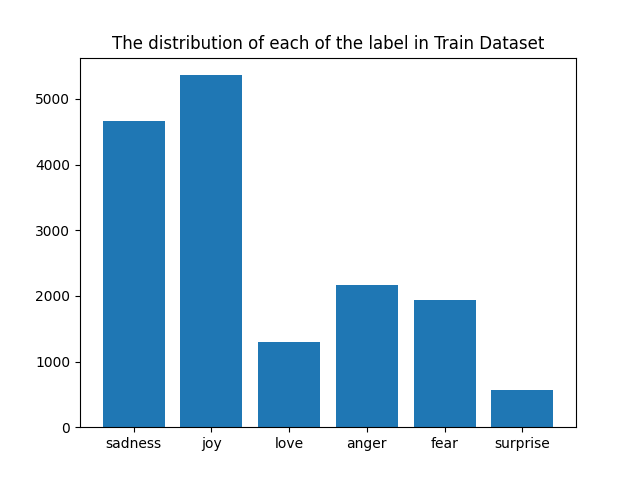
\includegraphics[scale=0.5]{Figures/dataset_distribution.png}}
    \caption{The graph for the distribution of each label in Train dataset}
    \label{fig:dataset}
\end{figure}

The distribution of each label for train dataset is not equal, the most being joy and the least being surprise. The Figure[\ref{fig:dataset}] will show the distribution of train dataset. 

\section{Methods}

\subsection{MiniLM}



\subsection{Llama2}
  
\subsection{RoBERTa}

\subsection{GPT-2}


